\documentclass[xelatex,ja=standard,a4paper,10pt,twocolumn]{bxjsarticle}
\geometry{margin=18mm,top=20mm,bottom=22mm,columnsep=7mm}
\usepackage{amsmath,amssymb,mathtools,bm}
\usepackage{graphicx}
\usepackage{booktabs}
\usepackage{multirow}
\usepackage{tabularx}
\usepackage{array}
\usepackage{siunitx}
\usepackage{xcolor}
\usepackage{tikz}
\usetikzlibrary{arrows.meta,positioning,fit,shapes.geometric}
\usepackage{enumitem}
\usepackage{caption}
\usepackage{subcaption}
\usepackage{float}
\usepackage{placeins}
\usepackage{url}
\usepackage[
  colorlinks=true,
  linkcolor=blue!45!black,
  citecolor=blue!45!black,
  urlcolor=blue!55!black
]{hyperref}
\ifpTeX
  \usepackage{pxjahyper}
\fi
\usepackage[nameinlink,noabbrev]{cleveref}

\captionsetup{font=small,labelfont=bf}
\setlength{\emergencystretch}{2em}
\setlength{\parindent}{1em}
\setlength{\parskip}{0pt}
\setlist{nosep,leftmargin=1.8em}
\sisetup{
  detect-all,
  group-separator={,},
  group-minimum-digits=4,
  range-phrase={--},
  range-units=single
}

\newcommand{\pt}{p_{\mathrm{T}}}
\newcommand{\met}{E_{\mathrm{T}}^{\mathrm{miss}}}
\newcommand{\Htt}{H\rightarrow\tau^{+}\tau^{-}}
\newcommand{\Ztt}{Z\rightarrow\tau^{+}\tau^{-}}
\newcommand{\epssig}{\varepsilon_{\mathrm{sig}}}
\newcommand{\epsbkg}{\varepsilon_{\mathrm{bkg}}}
\DeclareSIUnit{\GeV}{GeV}
\DeclareSIUnit{\TeV}{TeV}
\newcommand{\code}[1]{\texttt{\detokenize{#1}}}
\newcommand{\todo}[1]{\textcolor{red!70!black}{[要確認: #1]}}

\crefname{figure}{図}{図}
\crefname{table}{表}{表}
\crefname{section}{節}{節}
\crefname{equation}{式}{式}

\hypersetup{
  pdftitle={再構成されたタウ対による等質量H/Z分離の探索},
  pdfauthor={Ryunosuke Baba}
}


\begin{document}

\twocolumn[
\begin{center}
  {\LARGE\bfseries
    再構成された \(\tau^{+}\tau^{-}\) 系による\\
    等質量 \(H/Z\) 分離の探索\par}
  \vspace{0.6em}
  {\large
    親ボソン横運動量を整合したATLAS高速シミュレーションに対する
    Transformer解析\par}
  \vspace{1.0em}
  {\large Ryunosuke Baba\par}
  \vspace{0.2em}
  {\small ICEPPサマースクール実習レポート\par}
  \vspace{0.2em}
  {\small 2026年7月30日\par}
\end{center}

\begin{minipage}{0.94\textwidth}
\small
\textbf{要旨}\quad
質量差を利用せずに \(\Htt\) と \(\Ztt\) を分離できるかを調べるため、
truthレベルの親ボソン質量をそれぞれ \(\SI{91.1872}{\GeV}\) と
\(\SI{91.1876}{\GeV}\) に設定した専用Monte Carlo標本を解析した。
予定したH/Z各500ファイルのうち、2026年7月29日時点で正常に読み出せた
631ファイル（63.1\%）を固定スナップショットとし、両標本に同じ再構成と
事象選択を適用した。事象選択では2本の再構成\(\tau\)候補を要求したが、
truth matchingや、候補が真のhadronic-\(\tau\)崩壊に対応することは
要求しなかった。標本を学習・検証・評価の3分割にあらかじめ固定し、
各分割でtruthレベルの親ボソン\(\pt\)を\(\SI{20}{\GeV}\)幅に区切って、
各区間のH/Z事象数を等しくした。
この処理により、親\(\pt\)のみを分類スコアとしたAUCは
\(0.5705\)から\(0.5007\)へ低下した。

再構成された\(\tau\)候補、飛跡、particle-flow object、missing transverse
momentumを可変長のtoken列として表し、双方向Transformerで分類した。
検証分割だけを用いてハイパーパラメータとepochを決めた最終モデルは、
56,338事象からなる固定評価分割でROC AUC \(0.6088\)、
binary cross entropy \(0.6749\)を得た。ただし、この分割は先行モデルの
評価にも使用済みであり、解析全体を通じて未見の独立holdoutではない。
また、標本全体のAUCに対する統計区間、学習seed間の変動、系統不確かさは
評価していない。したがって、本結果はスピン相関を単独で測定したものではなく、
固定した部分Monte Carlo標本に対する再構成候補分類の探索的な概念実証である。

\vspace{0.5em}
\textbf{キーワード}\quad
\(\tau\)レプトン、スピン相関、Transformer、Monte Carlo、事象分類
\end{minipage}
\vspace{1.2em}
]

\section{序論}
\label{sec:introduction}

\(\tau\)レプトンは寿命が短く、検出器内で直接観測される前に崩壊する。
一方で、その崩壊粒子の運動学分布は親\(\tau\)の偏極に依存する。
したがって、\(\tau^{+}\tau^{-}\)対の崩壊生成物を組み合わせることで、
親粒子のスピンや結合構造に感度を持ち得る
\cite{TauSpinner,TauSpinML}。
この性質は、スカラー粒子であるHiggsボソンとベクトル粒子である\(Z\)ボソンを
\(\tau\tau\)終状態で比較する動機になる。

通常の標準模型の \(H\) と \(Z\) では質量が大きく異なるため、
再構成量を用いた分類器は、スピン相関を使わずとも質量やそれと相関する
運動学量から両者を分離できる。本研究ではこの自明な差を抑えるため、
Higgs状スカラー \(H\) と\(Z\)の生成質量をともに約
\(\SI{91.2}{\GeV}\)へ設定した専用Monte Carlo標本を用いる。
これは\(\SI{125}{\GeV}\)の標準模型Higgsボソンを測定する解析ではなく、
ほぼ同じ質量を持つスカラー状の \(H\) 標本と、ベクトル粒子 \(Z\) の
標本を比較するものである。
さらに、初期診断で見つかった親ボソン\(\pt\)の差を抑えるため、
truth情報に基づき、幅\(\SI{20}{\GeV}\)の各\(\pt\)区間で
H/Z事象数を等しくする。

この条件の下で、再構成されたhadronic-\(\tau\)候補、それらに対応する
trackとPFO、および事象全体の\(\met\)をTransformer
\cite{Transformer}へ入力する。Transformerは可変長の構成要素を
同一事象内で直接関連付けられるため、固定長の高レベル変数へ情報を
圧縮せずに、\(\tau\)崩壊の多次元相関を扱うことができる。

本稿では、まず使用した標本と再構成を\cref{sec:samples}で述べる。
\cref{sec:method}では\(\pt\)整合、入力表現、学習とモデル選択を
定義し、\cref{sec:results}で最終性能を示す。
最後に\cref{sec:discussion}で、結果から言えることと、スピン相関へ
帰属する前に必要な検証を分けて議論する。

\section{Monte Carlo標本と事象再構成}
\label{sec:samples}

\subsection{専用 \(H/Z\rightarrow\tau\tau\) 標本}

入力は、\(H+j\)および\(Z+j\)生成と\(\tau\)崩壊を分けて作り、
Les Houches Eventを結合した専用標本である。
重心系エネルギーは\(\sqrt{s}=\SI{13}{\TeV}\)である。
production過程にはMadGraph 3.5.5
\cite{MadGraph5}、parton showerにはPythia 8.312
\cite{Pythia82}、heavy-flavour decayにはEvtGen 2.2.1
\cite{EvtGen}を用いた。
ntupleで確認したtruth親ボソン質量は、H標本が
\(\SI{91.1872}{\GeV}\)、Z標本が\(\SI{91.1876}{\GeV}\)であり、
解析の目的に対して同一質量とみなせる設定である。
production側にはpartonの\(\pt>\SI{200}{\GeV}\)という生成条件がある。
\(\tau\)崩壊にはTauDecay UFO \cite{TauDecay}を用いた。
生成記録では、生成段階のスピン相関を崩壊粒子へ伝える構成とされている。
ただし、本稿の作成時点で生成カード、coupling設定、摂動次数、
decay/filter条件をrepository内の固定成果物として回収できなかったため、
その設定を本解析内で独立に検証したとはみなさない。

検出器応答にはATLASのAtlFast3
\cite{ATLASDetector,AtlFast3}を用いた。
入力metadataは\code{ATLFAST3_QS}、campaignは\code{mc20e}、
AMI tagは\code{r14861}である。再構成後の入力形式は
\code{DAOD_PHYS}である。private production directoryでは999801と999802を
標本識別子として用いたが、これらを公式DSIDとはみなさない。
ntupleの\code{mcChannelNumber}は両標本とも999999であり、
H/Zは標本名とtruth親ボソンPDG ID 25/23で監査した。
parton distribution functionとtuneも固定スナップショットのmetadataから
追跡できなかった。したがって、生成段階を含む完全な再現性は主張せず、
本稿の再現性の対象を固定DAOD以降の処理に限定する。

標本全体の生成完了を待たず、2026年7月29日21時59分時点で
正常に開けたDAODを\code{fixed-partial-v2}として凍結した。
予定していたH/Z各500ファイルに対し、Hは331ファイル、Zは300ファイルであり、
全体の63.1\%に相当する。Hの1ファイルは生成途中でcloseされておらず、
ROOTで開けなかったため除外した。
\cref{tab:sample_counts}に入力数と事象選択後の数を示す。
全64 HTCondorジョブはreturn code 0で完了し、出力64 ROOTファイルは
すべて読み取り可能であった。H/Zで84ブランチのschemaが一致し、
truth親ボソンPDG IDの不一致は0であった。

\begin{table*}[t]
  \centering
  \caption{固定スナップショット\code{fixed-partial-v2}の事象数。
    選択効率は選択後entry数を、実際に読み取れたraw事象数で割った値である。}
  \label{tab:sample_counts}
  \begin{tabular}{lrrrrr}
    \toprule
    標本 & private ID & DAODファイル & raw事象 & 選択後事象 & 選択効率 \\
    \midrule
    \(H\rightarrow\tau\tau\) & 999801 & 331 & 661,964 & 332,932 & 50.29\% \\
    \(Z\rightarrow\tau\tau\) & 999802 & 300 & 599,955 & 306,731 & 51.13\% \\
    \midrule
    合計 & --- & 631 & 1,261,919 & 639,663 & 50.69\% \\
    \bottomrule
  \end{tabular}
\end{table*}

\subsection{\(\tau\)候補と事象選択}
\label{subsec:selection}

再構成にはAnalysisBase 25.2.32のCommon Physics処理を用いた。
\code{TauJets}から解析用copyを作り、energy calibrationとselectionを
H/Zへ共通に適用した。hadronic-\(\tau\)の再構成と同定の一般的な考え方は
Ref.~\cite{ATLASTauID}にまとめられている。
本解析の具体的な選択を\cref{tab:selection}に示す。
条件を通る候補がちょうど2本で、かつopposite-signである事象だけを残した。
出力では負電荷側を\(\tau_0=\tau^-\)、正電荷側を
\(\tau_1=\tau^+\)とする。
truth matchingまたはtruth hadronic-decay flagは選択に要求せず、
trigger requirementも設けていない。
そのため、\cref{tab:sample_counts}の効率はraw DAOD事象を分母とする
処理上の通過率であり、真の
\(\tau_{\mathrm{had}}\tau_{\mathrm{had}}\)信号効率ではない。
0本、1本、2本のtruth-matched \(\tau\)候補の割合やfake組成は
この固定スナップショットでは監査していない。

\begin{table}[t]
  \centering
  \caption{解析に用いた\(\tau\)候補および事象選択。}
  \label{tab:selection}
  \small
  \begin{tabular}{ll}
    \toprule
    項目 & 条件 \\
    \midrule
    入力container & \code{TauJets} \\
    \(\tau\) transverse momentum & \(\pt\geq\SI{20}{\GeV}\) \\
    \(\tau\) pseudorapidity & \(|\eta|\leq 2.5\) \\
    \(\tau\) charge & \(|q|=1\) \\
    track multiplicity & 1または3 \\
    jet rejection & RNN Loose \\
    \(\eta\) crack veto & なし \\
    \(\phi\) requirement & なし \\
    candidate multiplicity & 条件通過候補がちょうど2本 \\
    pair charge & opposite-sign \\
    \bottomrule
  \end{tabular}
\end{table}

入力DAODにはGNTau v0のscoreとflagが保存されていたが、
AnalysisBase 25.2.32の標準GNTau selectionが要求する
\code{GNTauL_v1trunc}とは互換でなかった。そのため、GNTau flagを
標準Loose selectionと同一視せず、本解析の選択にはRNN Looseを使った。
GNTau/RNNの連続スコアは診断用ブランチとして保存し、一部はNN入力へ用いた。

入力DAODには保存済みFinal \(\met\) termがなかった。
そこで、\code{MET_Core_AntiKt4EMPFlow}、
\code{METAssoc_AntiKt4EMPFlow}および較正済みのelectron、muon、
photon、jet、\(\tau\)を用いて、CPのMissingET blockから
\code{AnaMET_NOSYS["Final"]}を再構成した。
標準Overlap Removalも同時に実行した。
処理は公称設定のみで、object efficiency scale factorと系統変動は
適用していない。
FastSim専用のtau smearing recommendationがない補正については、
FullSim recommendationへfallbackする警告が記録された。

\subsection{解析ntuple}

自作の\code{TauSpinNtupleAlg}は、選択を通過した1事象を
TTree \code{tauspin}の1 entryとして保存する。事象およびFinal \(\met\)、
2本の\(\tau\) summary、各\(\tau\)に対応する可変長trackとPFO、
vertex、truth診断を合わせて84ブランチを持つ。
truthブランチは標本監査、親\(\pt\)整合およびラベル確認に使うが、
分類器の入力には使わない。

固定スナップショットのntuple生成では全ジョブが終了したものの、
MetMakerからsoft termに重複する可能性のあるobjectがmissingである旨の
messageが20ジョブに計24行記録された。また、全64ジョブでinvalidな
tau-track linkをskipした旨の警告が少なくとも1回記録されており、
事象単位の発生頻度は監査していない。これらはジョブの失敗や
非有限なFinal \(\met\)には
直結しなかったが、
保存済みFinal \(\met\)を持つ標準DAODとの数値比較は未実施である。
この点は最終的なdetector-level性能を解釈する際の制約として残す。

\section{解析手法}
\label{sec:method}

\subsection{データ分割と親ボソン \(\pt\) の整合}
\label{subsec:matching}

H/Zのntupleを、決定的ハッシュにより学習、検証、評価へ
80:10:10で先に分けた。成果物では各分割をそれぞれ
\code{train}、\code{validation}、\code{test}と呼ぶ。
ただし、最後の分割は先行モデルの確認にも使われたため、本稿では
解析全体を通じて未見の評価標本ではなく、\emph{固定評価分割}と位置付ける。

同じ標本内で\code{eventNumber}が重複したため、標本名 \(S\)、ROOTファイルの
basename \(F\)、ファイル内entry番号 \(i\)から
\begin{equation}
  K=\code{42}:S:F:i
  \label{eq:split_key}
\end{equation}
という文字列を作った。この文字列のBLAKE2b digestを8 byteで計算し、
big-endian整数を\(2^{64}\)で割った値を \(u\in[0,1)\) とした。
\(u<0.8\)を学習、\(0.8\leq u<0.9\)を検証、残りを固定評価分割へ
割り当てた。この定義は同じファイル構成からは再現するが、ROOTファイルを
再分割または再結合すると変化し得る。

分割後、それぞれの分割内でtruth親ボソン\(\pt\)を
\(\SI{20}{\GeV}\)幅に分けた。\(\SI{1000}{\GeV}\)以上は1個の
overflow区間とした。分割 \(s\)、区間 \(i\)で保持するH/Z事象数を
\begin{equation}
  N^{\mathrm{keep}}_{s,i}
  = \min\left(N^{H}_{s,i},N^{Z}_{s,i}\right)
  \label{eq:pt_matching}
\end{equation}
とし、seed 42と同じ事象識別子から得た16 byteのBLAKE2b rankに従って、
各クラスを決定的にdownsamplingした。この処理が保証するのは、
各分割の\(\SI{20}{\GeV}\)区間ごとにH/Zの事象数が等しいことだけである。
各区間およびoverflow区間内部の分布形状まで一致させるものではない。
整合前後の事象数と診断結果は\cref{subsec:matching_result}に示す。

\subsection{入力表現と前処理}
\label{subsec:features}

入力事象を次の可変長token列へ変換した。
\begin{equation}
\begin{split}
  [\mathrm{CLS}], [\mathrm{EVENT}],&
  [\tau^-], [\mathrm{TRACK}^- \ldots], [\mathrm{PFO}^- \ldots],\\
  &[\tau^+], [\mathrm{TRACK}^+ \ldots], [\mathrm{PFO}^+ \ldots].
\end{split}
\label{eq:token_sequence}
\end{equation}
trackとPFOは各\(\tau\)側で\(\pt\)降順に並べた。
事象ごとにtoken数が異なるため、保存時はpaddingせず、
mini-batch内の最大長までdynamic paddingし、padding maskを用いた。

入力の概要を\cref{tab:features}に示す。
Relative-v3表現では、絶対的な再構成量に加え、track/PFOと親\(\tau\)の
相対座標、\(\tau\)対の相対量、各\(\tau\)と\(\met\)の角度差を加えた。
truth量、標本識別子、event/run番号、primary vertex座標は入力から除いた。

\begin{table*}[t]
  \centering
  \caption{Relative-v3のtoken別入力。次元は前処理後に各projectorへ渡す
    連続特徴量の数であり、decay-mode categoryは別embeddingで加える。
    変換後の全特徴量名と順序は\cref{app:features}に示す。}
  \label{tab:features}
  \small
  \begin{tabularx}{\textwidth}{@{}l c X@{}}
    \toprule
    token & 次元 & 主な入力 \\
    \midrule
    EVENT & 13 &
      Final \(\met\)、\(\phi(\met)\)、sum \(E_{\mathrm{T}}\)、
      \(\tau\)対の\(|\Delta\eta|\)、\(\sin/\cos\Delta\phi\)、
      \(\log(\pt^{\tau^-}/\pt^{\tau^+})\)、
      \(\met\)と各\(\tau\)の\(\sin/\cos\Delta\phi\)、
      \(\met/(\pt^{\tau^-}+\pt^{\tau^+})\) \\
    TAU & 10 &
      \(\pt,\eta,\phi,m\)、track数、isolation track数、
      RNN/GNTauスコア、vertex \(\Delta z\)。
      decay modeはcategory embedding \\
    TRACK & 19 &
      \(\pt,\eta,\phi,q,d_0,z_0\sin\theta\)、track分類flag、
      Pixel/SCT/TRT hit数、親\(\tau\)に対する
      \(\Delta\eta,\sin/\cos\Delta\phi,\log(1+\pt\mathrm{\ fraction})\) \\
    PFO & 10 &
      \(\pt,\eta,\phi,E\)、\(\pi^0\) flag、親\(\tau\)に対する
      \(\Delta\eta,\sin/\cos\Delta\phi,\log(1+\pt\mathrm{\ fraction})\) \\
    \bottomrule
  \end{tabularx}
\end{table*}

\(\phi\)と\(\Delta\phi\)は\(\sin\phi,\cos\phi\)へ変換した。
\(\pt\)、energy、mass、\(\met\)、sum \(E_{\mathrm{T}}\)は
\(\log(1+x/\SI{1}{\GeV})\)へ写し、その後に標準化した。
角度の\(\sin/\cos\)、charge、各種flagは標準化せず、それ以外の
連続特徴量には学習分割だけから求めた平均と標準偏差を用いた。
欠損値sentinel \(-999\)および\(-9999\)を許容せず、
非有限値も変換時に拒否した。検証分割と固定評価分割の情報は
前処理統計へ混ぜていない。全570,096事象について、Tensorの有限性、
ラベル、offset終端、shard内事象数を検証した。

\begin{figure*}[t]
  \centering
  \begin{tikzpicture}[
    node distance=12mm and 8mm,
    box/.style={
      draw=black!65, rounded corners=2pt, align=center,
      minimum height=12mm, text width=34mm, fill=blue!4,
      font=\small
    },
    decision/.style={
      draw=black!65, rounded corners=2pt, align=center,
      minimum height=12mm, text width=34mm, fill=orange!8,
      font=\small
    },
    arrow/.style={-{Latex[length=2.4mm]},thick,draw=black!65}
  ]
    \node[box] (daod) {専用 \(H/Z+j\)\\DAOD\_PHYS\\mass \(\simeq\SI{91.2}{\GeV}\)};
    \node[box,right=of daod] (reco) {共通CP再構成\\RNN Loose\\2本のOS \(\tau\)候補};
    \node[box,right=of reco] (split) {決定的な\\80:10:10分割};
    \node[decision,right=of split] (match) {各分割・truth \(\pt\)\\20 GeV区間で同数化};
    \node[box,below=of match] (tokens) {Relative-v3\\可変長token列\\動的padding};
    \node[box,left=of tokens] (model) {双方向\\Transformer\\\(H=1,\ Z=0\)};
    \node[decision,left=of model] (select) {検証分割のみで\\HPO・epoch選択};
    \node[box,left=of select] (test) {固定評価分割\\（成果物名test）\\AUC \(=0.6088\)};

    \draw[arrow] (daod) -- (reco);
    \draw[arrow] (reco) -- (split);
    \draw[arrow] (split) -- (match);
    \draw[arrow] (match) -- (tokens);
    \draw[arrow] (tokens) -- (model);
    \draw[arrow] (model) -- (select);
    \draw[arrow] (select) -- (test);
  \end{tikzpicture}
  \caption{解析の全体フロー。truth親ボソン\(\pt\)は区間ごとの事象数整合にのみ使い、
    Transformerへは入力しない。ハイパーパラメータと最終epochは
    検証分割だけで固定した。固定評価分割は成果物中の\code{test}に相当するが、
    先行モデルにも使用済みであり、未見の評価標本ではない。}
  \label{fig:workflow}
\end{figure*}

\subsection{Transformerと学習}

EVENT、TAU、TRACK、PFOには種類ごとに独立なlinear projectorを用い、
共通のhidden dimensionへ写した。これにobject-type embedding、
\(\tau\)-side embedding、\(\tau\) decay-mode embeddingを加えた。
通常のsequence positional encodingは使用しない。
encoderは双方向であり、causal maskも用いない。
\([\mathrm{CLS}]\)の最終hidden stateを2層MLPへ入力し、
\(H=1\)、\(Z=0\)の1 logitを出力する。
探索した5種類のmodel profileは\cref{app:hpo_details}に示す。

損失関数には\code{BCEWithLogitsLoss}を用い、学習時はH/Zを均等に
samplingした。MC事象weightは使用していない。
optimizerはAdamW、weight decay \(10^{-4}\)、batch size 128、
random seed 42とし、TF32で学習した。

\subsection{HPOとモデル選択}
\label{subsec:model_selection}

Optuna \cite{Optuna}のTPE samplerを用い、model profile、learning rate、
dropout、schedulerを探索した。sampler seedは42、最初の7 trialは
anchor設定であり、trial間の途中pruningには\code{NopPruner}を用いた。
目標は最大100 trialであったが、新規trialの開始期限を
2026年7月30日06時45分（JST）に設定した。各trialの上限は32 epochである。
探索範囲を\cref{tab:hpo_space}に示す。

HPO中は固定評価分割を読み込まず、全検証事象のAUCだけを用いた。
目的関数は、中央epochが8以降となる連続3 epochの検証AUC平均の最大値とし、
最大windowの中央epochのcheckpointを保存した。
各trialは20 epochまで停止せず、epoch 21以降に限って次の停止を許した。
3-epoch平均AUCが少なくとも0.0005改善しない状態が6 epoch続けば
plateau、同平均AUCが最良値から0.003以上低く、かつ同平均lossが
最良windowより悪い状態が3 epoch続けばoverfitと判定した。

\begin{table}[t]
  \centering
  \caption{HPOの探索範囲。model profileの各層次元は
    \cref{app:hpo_details}に示す。weight decay、batch size、seedは
    それぞれ\(10^{-4}\)、128、42に固定した。}
  \label{tab:hpo_space}
  \small
  \begin{tabularx}{\columnwidth}{@{}l X@{}}
    \toprule
    parameter & 探索範囲 \\
    \midrule
    profile & Small、Current、Deep、Wide、Large \\
    learning rate & \(7\times10^{-5}\)--\(2\times10^{-4}\)（log scale） \\
    dropout & 0--0.25 \\
    scheduler & constant、cosine decay + 5\% warmup \\
    \bottomrule
  \end{tabularx}
\end{table}

完了trialには3-epoch平均AUCを主指標とする選択規則を適用した。
首位との差が0.001未満なら最小validation loss、さらに同程度なら
パラメータ数の小さい方を優先した。この順位規則は実行時の
\code{study_config.json}に保存されていないため、事前登録済みとはみなさず、
検証結果だけに基づく事後的なモデル選択規則として扱う。

\section{結果}
\label{sec:results}

\subsection{\(\pt\) 整合の診断}
\label{subsec:matching_result}

\cref{tab:split_counts}に整合前後の事象数を示す。
全体の保持率はHで85.62\%、Zで92.93\%であった。
truthレベルの親ボソン\(\pt\)のみを分類スコアとしたROC AUCは、
整合前の0.5705から整合後の0.5007へ低下した。
これは、\(\pt\)に関する単調な一次元の順位差が小さくなったことを示す。
一方、各\(\SI{20}{\GeV}\)区間内の分布形状、overflow区間内の差、
または非単調な
\(\pt\)依存の識別力を除外する検定ではない。

\begin{table*}[t]
  \centering
  \caption{決定的な80:10:10分割とtruth親ボソン\(\pt\)整合の前後における
    事象数。各分割の\(\SI{20}{\GeV}\)区間ごとに少数クラスの数を残し、
    \(\pt\geq\SI{1000}{\GeV}\)は一つのoverflow区間とした。
    ``test''は56,338事象の固定評価分割を表す。}
  \label{tab:split_counts}
  \begin{tabular}{lrrrrrr}
    \toprule
    & \multicolumn{3}{c}{整合前} & \multicolumn{3}{c}{整合後} \\
    \cmidrule(lr){2-4}\cmidrule(lr){5-7}
    split & H & Z & 合計 & H & Z & 合計 \\
    \midrule
    train      & 266,685 & 245,519 & 512,204 & 228,360 & 228,360 & 456,720 \\
    validation &  33,312 &  30,693 &  64,005 &  28,519 &  28,519 &  57,038 \\
    test       &  32,935 &  30,519 &  63,454 &  28,169 &  28,169 &  56,338 \\
    \midrule
    合計       & 332,932 & 306,731 & 639,663 & 285,048 & 285,048 & 570,096 \\
    \bottomrule
  \end{tabular}
\end{table*}

\subsection{HPOとモデルプロファイルの選択}

開始期限までに21回のtrialが完了し、そのうち18回はtrial内の
early stoppingによって終了した。完了trialに前節の順位規則を適用し、
trial 5を選択した。
その設定と観測された目的関数を\cref{tab:hpo_selected}に示す。
trial 5の目的関数は0.604504であり、順位規則上の2位trial 13との差は
0.000156にすぎない。したがって、trial 5を一意な最適点とは解釈しない。

\begin{table}[t]
  \centering
  \caption{検証分割だけを用いて選択したtrial 5の設定。
    objectiveは中央epochが8以降となる3-epoch平均検証AUCの最大値である。}
  \label{tab:hpo_selected}
  \small
  \begin{tabular}{lr}
    \toprule
    項目 & trial 5 \\
    \midrule
    profile & Current \\
    \(d_{\mathrm{model}}\) / heads / layers & 128 / 8 / 4 \\
    feed-forward dimension & 512 \\
    learning rate & \(10^{-4}\) \\
    dropout & 0.10 \\
    scheduler & cosine + 5\% warmup \\
    trainableパラメータ数 & 819,201 \\
    objective & 0.604504 \\
    \bottomrule
  \end{tabular}
\end{table}

\begin{figure*}[t]
  \centering
  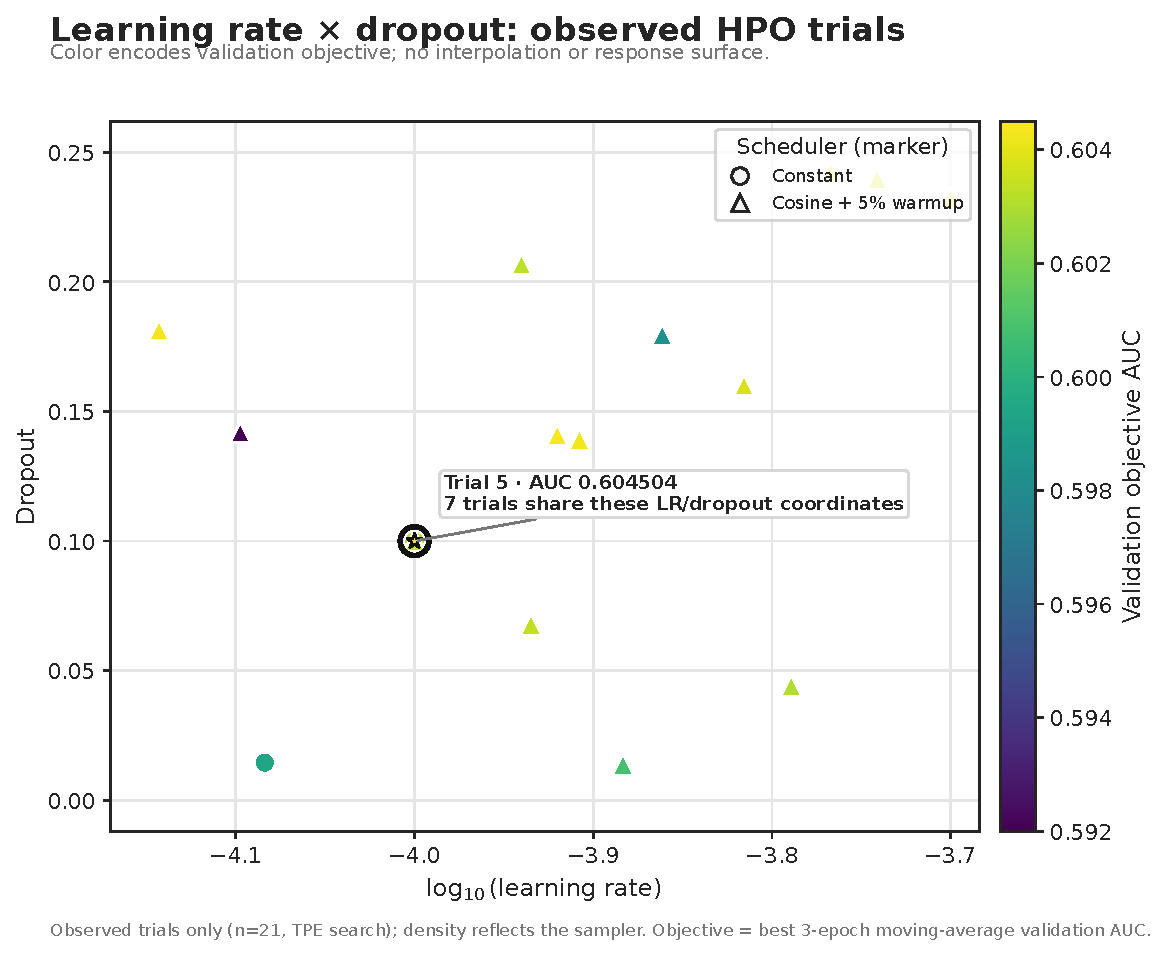
\includegraphics[width=0.78\textwidth]{figures/lr_dropout_objective_scatter.pdf}
  \caption{固定した部分標本の検証分割で実行した21回のHPO trial。
    横軸はlearning rate、縦軸はdropout、色は最大3-epoch平均検証AUC、
    markerはschedulerを示す。星が選択したtrial 5である。
    同じ座標には7個のanchor trialが重なる。TPEの探索点は一様標本では
    ないため、点密度を性能の確率密度とは解釈せず、補間面も描かない。}
  \label{fig:hpo}
\end{figure*}

\subsection{40 epoch最終学習}

HPOで固定したtrial 5の設定を使い、early stoppingを無効にして
40 epochの最終学習を最初から実行した。
cosine schedulerは総step数に依存するため、32 epochのHPO checkpointは
延長せず、40 epochを学習期間とする独立の再学習を行った。

連続3 epochのvalidation AUC平均はepoch 23--25で最大
0.6045となった。その中央であるepoch 24を、最終再学習モデルを
固定評価分割へ適用する前にcheckpointとして固定した。
epoch 24のvalidation AUCは0.6047、lossは0.6771である。

\cref{fig:learning_curve}に学習履歴を示す。
epoch 24から40にかけて、学習損失は0.6693から0.6643へ低下した一方、
検証損失は上昇し、検証AUCも0.6047から0.6024へ
低下した。すなわち、学習標本への適合が進む一方で検証性能は悪化しており、
epoch 24以降は過学習と判断した。

\begin{figure*}[t]
  \centering
  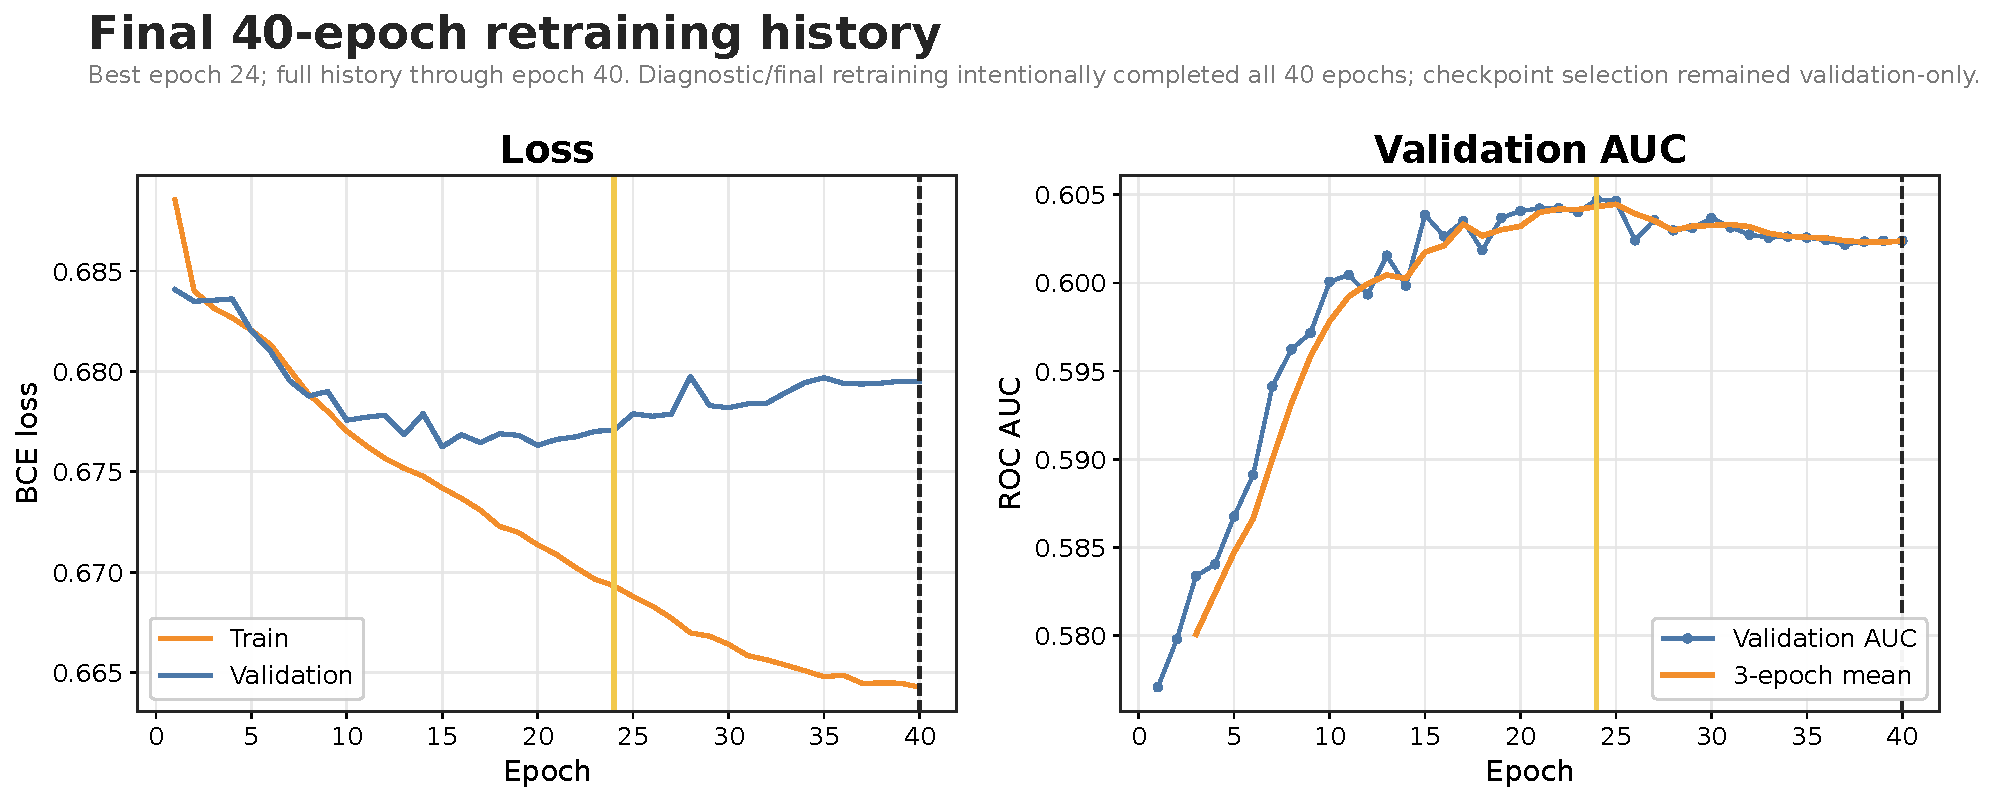
\includegraphics[width=0.94\textwidth]{figures/learning_curve_combined.pdf}
  \caption{trial 5設定を用いた456,720学習事象での40 epoch再学習。
    左はepochごとの学習/検証BCE loss、右は57,038検証事象の
    ROC AUCと3-epoch平均である。黄色線は検証AUCだけから選択した
    epoch 24、黒破線は学習終端を表す。epoch 24以降は学習損失が
    低下する一方、検証損失とAUCは悪化する。}
  \label{fig:learning_curve}
\end{figure*}

\subsection{最終分類性能}

選択したcheckpointを再読み込みし、validation AUCとlossが
保存時の値と一致することを確認した（差0）。その後、固定した最終モデルを56,338事象の
固定評価分割へ適用した。この分割はHPO中には読み込んでいないが、
先行するtrial 5モデルの評価に一度用いた後で40 epoch再学習を行っている。
したがって、以下は解析全体から独立した未見標本の性能推定ではなく、
固定評価分割上の記述値である。
結果を\cref{tab:final_metrics}に示す。
ROC AUCは0.6088、BCE lossは0.6749であった。
検証分割の点推定値とは近いが、標本全体のAUCとlossに対する統計区間を
評価していないため、両者の統計的な整合性検定は行っていない。

\begin{table}[t]
  \centering
  \caption{epoch 24最終モデルの検証分割と固定評価分割における性能。
    Hを信号、Zを背景とする。70\%信号効率の値は各分割のROC上で
    最初に到達する点を分割ごとに読み取った記述値であり、統計区間は
    付していない。固定評価分割は成果物中の\code{test}である。}
  \label{tab:final_metrics}
  \small
  \begin{tabular}{lrr}
    \toprule
    指標 & 検証 & 固定評価 \\
    \midrule
    事象数 & 57,038 & 56,338 \\
    ROC AUC & 0.604712 & 0.608814 \\
    BCE loss & 0.677076 & 0.674915 \\
    \(\epssig\) & 0.700025 & 0.700025 \\
    \(\epsbkg=\varepsilon_Z\) & 0.560188 & 0.548972 \\
    \(1/\varepsilon_Z\) & 1.78512 & 1.82159 \\
    \bottomrule
  \end{tabular}
\end{table}

固定評価分割のROC上で\(\epssig\geq0.70\)を初めて満たす点は、
分類スコアの閾値0.4658に対応した。
そのとき\(\epssig=0.7000\)、\(\epsbkg=0.5490\)、
背景除去率\(1/\epsbkg=1.8216\)であった。
ここで信号はHクラス、背景はZクラスであり、この値は
jet、top-quark過程などに対する背景除去率ではない。
この閾値は固定評価分割のスコアから読み取ったものであり、
検証分割で固定して評価分割へ移した動作点ではない。
したがって、本稿ではROC曲線上の記述的な性能点としてのみ扱う。

\begin{figure*}[t]
  \centering
  \begin{subfigure}[t]{0.49\textwidth}
    \centering
    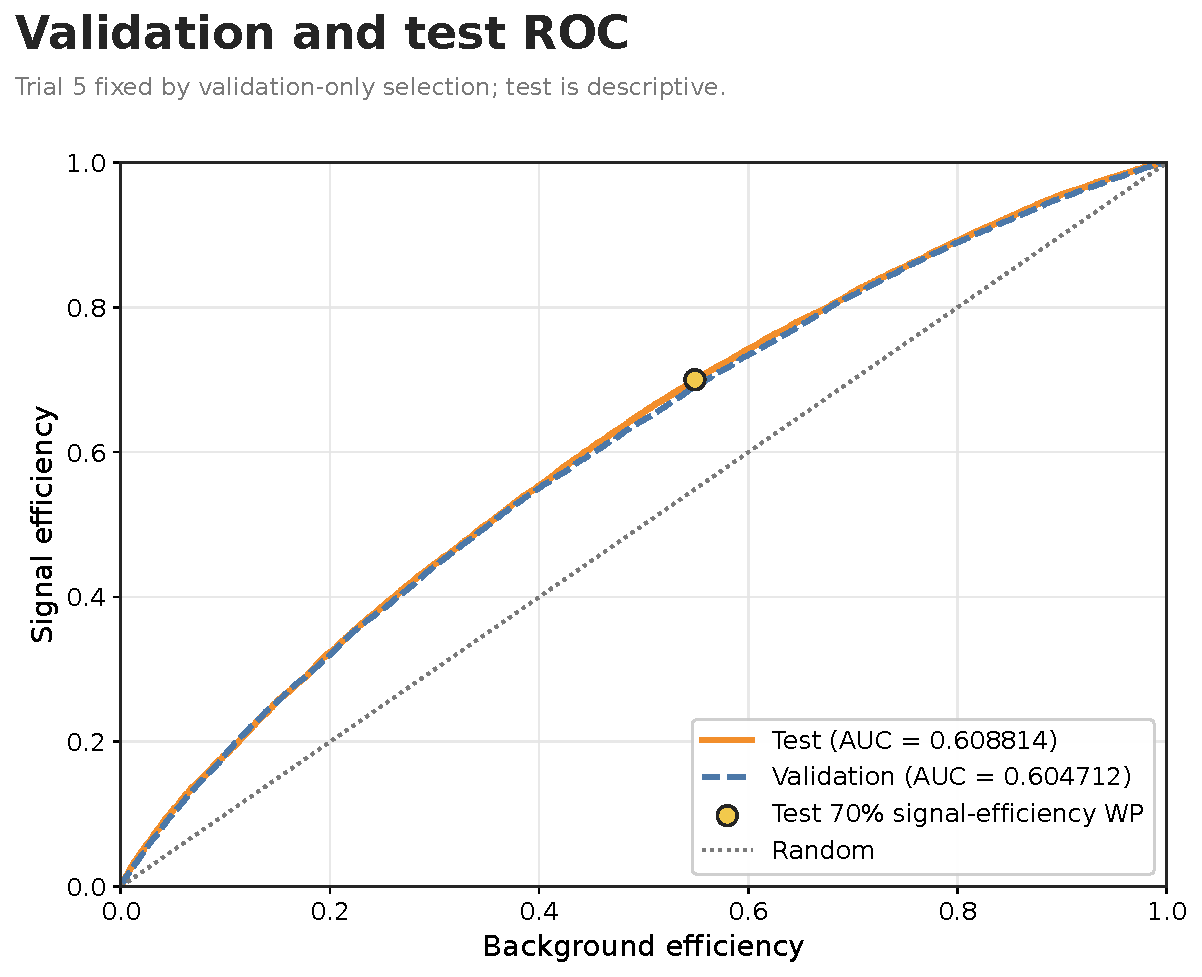
\includegraphics[width=\textwidth]{figures/roc_val_vs_test.pdf}
    \caption{検証分割と固定評価分割のROC。横軸はZ効率、
      縦軸はH効率であり、黄色点は固定評価ROC上でH効率70\%となる記述点。}
    \label{fig:roc}
  \end{subfigure}
  \hfill
  \begin{subfigure}[t]{0.49\textwidth}
    \centering
    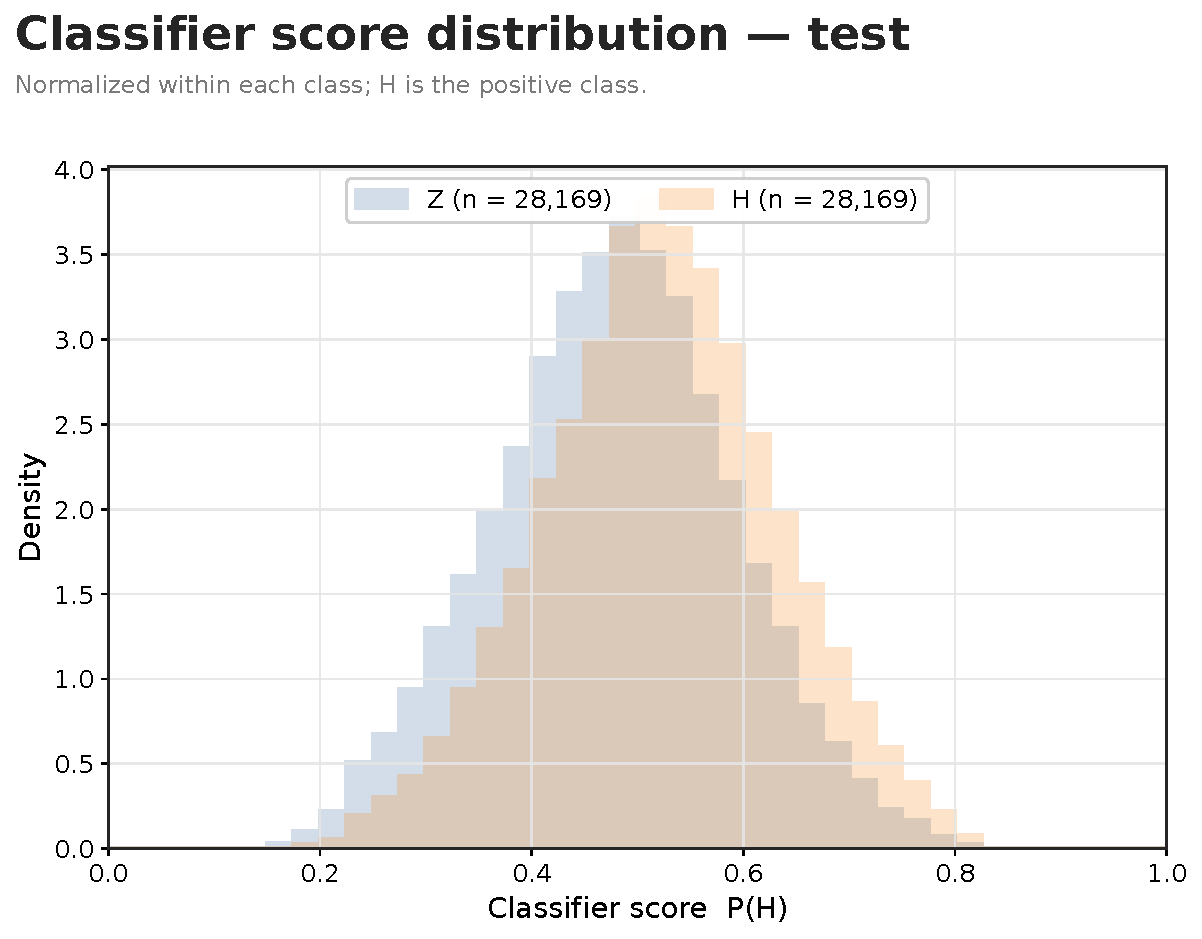
\includegraphics[width=\textwidth]{figures/score_distribution_test.pdf}
    \caption{固定評価分割のH/Z別スコア \(s=\sigma(\mathrm{logit})\)分布。
      各クラスで単位面積に規格化した。\(s\)の確率calibrationは未評価。}
    \label{fig:scores}
  \end{subfigure}
  \caption{epoch 24モデルの分類性能。左は57,038検証事象と56,338固定評価事象の
    ROC、右は固定評価事象のクラス別規格化スコア分布である。
    H/Z分布は大きく重なるが、Hは高スコア側、Zは低スコア側へずれる。
    左図の70\%信号効率点は固定評価ROC上で読み取った記述点である。}
  \label{fig:classification}
\end{figure*}

\subsection{親ボソン \(\pt\) 依存性}

\cref{fig:pt_auc}に固定評価分割AUCのtruth親ボソン\(\pt\)依存性を示す。
中央領域では整合に用いた\(\SI{20}{\GeV}\)区間を保ち、
低統計となる\(\pt<\SI{180}{\GeV}\)と
\(\pt\geq\SI{460}{\GeV}\)はそれぞれ統合した。
誤差棒はクラス別に層化したbootstrapを1000回行って得た
16--84パーセンタイル区間であり、有限な固定評価標本による統計変動の目安である。

多くの区間でAUCはおよそ0.59--0.63に分布し、
親\(\pt\)に対する単調な増減は見られない。
\(\pt<\SI{180}{\GeV}\)ではAUCが0.5528と低い一方、
高\(\pt\)側は事象数が少なく区間も広い。
区間間の差に対するlook-elsewhere効果や系統不確かさは
評価していないため、局所的な上下を物理効果として解釈しない。

\begin{figure*}[t]
  \centering
  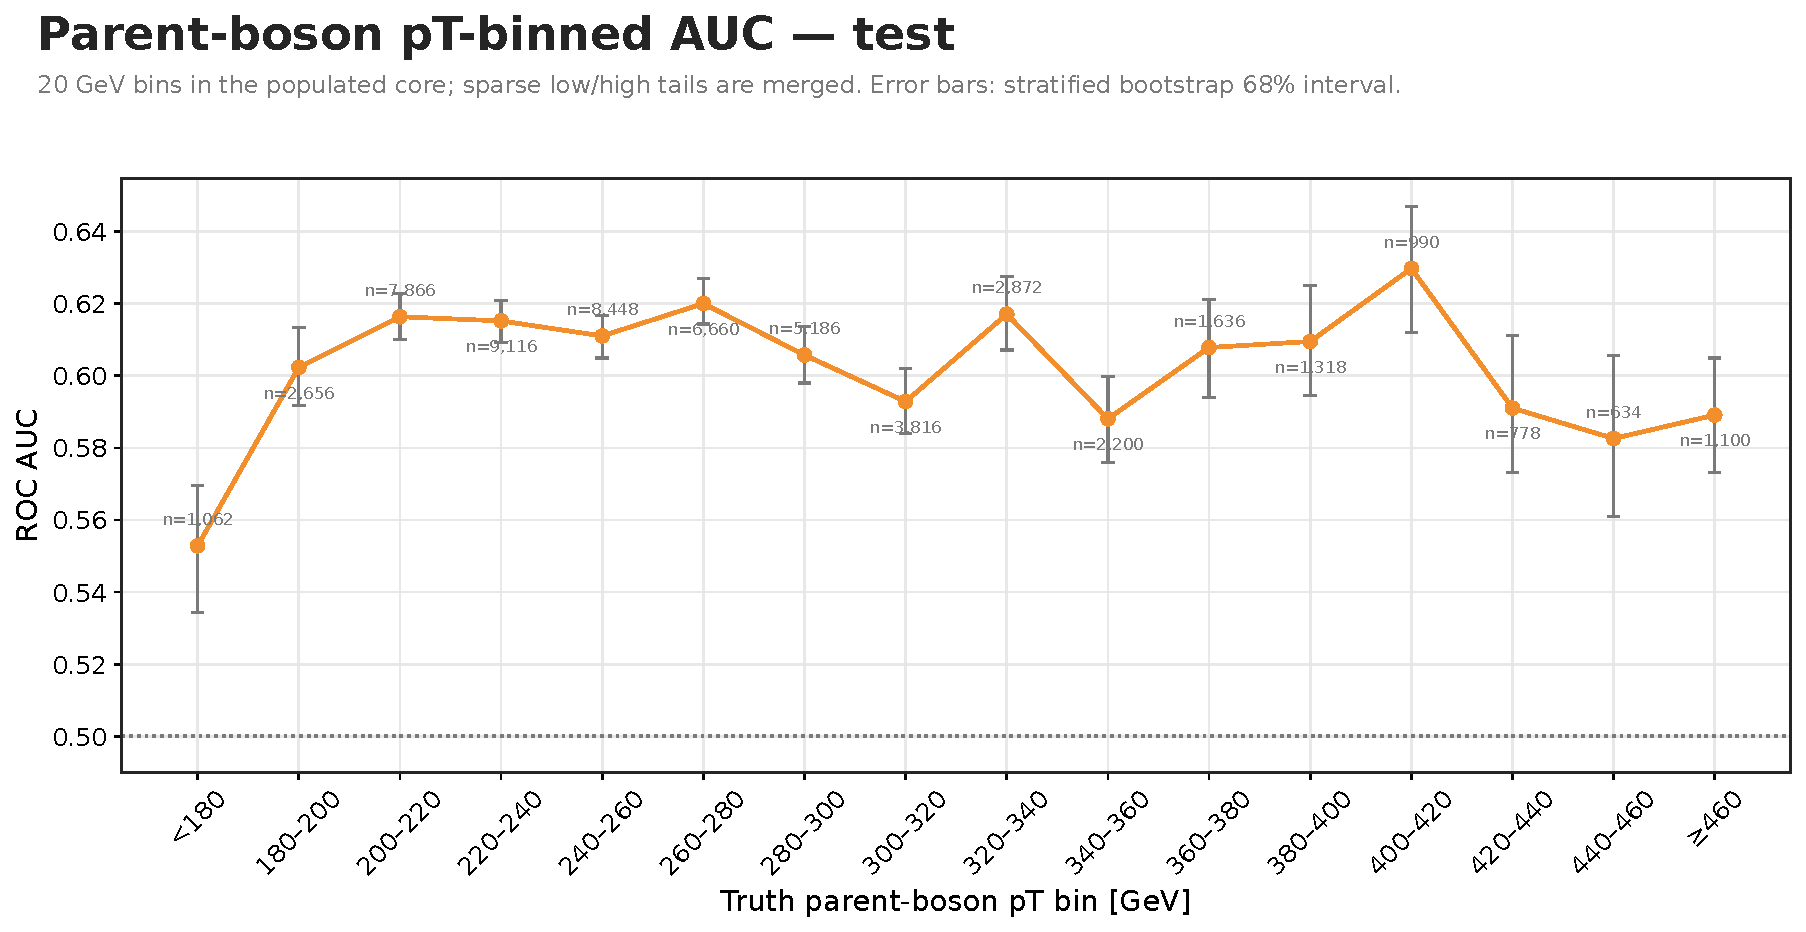
\includegraphics[width=0.78\textwidth]{figures/pt_binned_auc_test.pdf}
  \caption{56,338事象の固定評価分割におけるtruth親ボソン\(\pt\)区間別ROC AUC。
    H/Z事象数は各区間で等しい。中央部は\(\SI{20}{\GeV}\)幅とし、
    \(\pt<\SI{180}{\GeV}\)と\(\pt\geq\SI{460}{\GeV}\)の疎なtailは
    それぞれ統合した。誤差棒はクラス別に層化したbootstrap 1000回の
    16--84パーセンタイル区間であり、系統不確かさを含まない。}
  \label{fig:pt_auc}
\end{figure*}

\FloatBarrier
\section{物理解釈と解析上の制約}
\label{sec:discussion}

\subsection{結果が示すこと}

親ボソンの質量は生成段階でほぼ揃え、さらにtruth親\(\pt\)について
各分割・\(\SI{20}{\GeV}\)区間のH/Z事象数を等しくした。
整合後に親\(\pt\)のみから求めたAUCが0.5007まで低下したことは、
単調な\(\pt\)順位差が主要な識別源ではないことと整合する。
ただし、各区間内の分布形状や非単調な依存は検定していないため、
最終AUC 0.6088に対する親\(\pt\)の寄与を完全に排除したとは言えない。
観測された分離は、再構成された\(\tau\)候補の運動学、構成要素、
impact parameter、IDスコア、\(\met\)、およびそれらの相対量の
少なくとも一部に、H/Zラベルと相関する多次元情報が残っていることを示す。

\(\tau\)崩壊粒子の分布が偏極とスピン相関を反映することは
よく知られており\cite{TauSpinner,TauSpinML}、本結果の一部がその情報に
由来することは物理的に期待できる。しかし、今回の分類器は、
理論的に定義されたスピン観測量だけを入力しているわけではない。
さらに、選択した2本の再構成\(\tau\)候補についてtruth matchingと
hadronic-\(\tau\)組成を監査しておらず、偽\(\tau\)候補の組成差も
識別源になり得る。
したがって、AUC 0.6088を「スピンだけによる分離能」と同一視することは
できない。本研究で直接示したのは、\emph{ほぼ等質量で、親\(\pt\)を
粗い区間ごとに同数化した専用標本において、広い再構成候補情報を使う
TransformerがH/Zラベルを分離した}ことである。

\subsection{統計・系統誤差}

本解析では標本全体のAUC、BCE loss、背景除去率に対する統計区間を
評価していない。示したbootstrap区間は\(\pt\)区間別AUCだけを対象とする。
また、detector calibration、tau ID、track/PFO、MET、pile-up、
generator、shower、PDFなどの系統変動も処理していない。
object efficiency scale factorとMC event weightも使用していない。
H/Zは等数へdownsampleした重みなしクラスとして扱っており、
断面積、積分ルミノシティ、期待事象数、significanceは
計算していない。
したがって、ここで示した数値は公称設定の特定Monte Carlo標本に対する
分類性能であり、実データ解析における期待感度や測定精度を表すものではない。

\subsection{標本と検証上の制約}

本研究の主な制約を次にまとめる。

\begin{enumerate}
  \item \textbf{\(\tau\)候補の組成}: 選択は再構成候補へ適用しており、
    0本、1本、2本のtruth-matched \(\tau\)を含む事象の割合と、真の
    hadronic-\(\tau\)対の割合をH/Z別に監査していない。偽候補または
    崩壊組成の差が識別力へ寄与し得るため、これはスピン解釈を妨げる。
  \item \textbf{部分標本}: 最終結果は予定した標本の63.1\%を固定した
    スナップショットに基づく。標本完成後には事象組成と学習曲線を
    再評価する必要がある。
  \item \textbf{残存する近道学習の可能性}: 整合したのはtruth親\(\pt\)だけである。
    各区間とoverflow区間の内部に残る分布形状、非単調な\(\pt\)依存、
    生成時の放射、\(\eta\)、jet recoil、再構成応答、
    崩壊モード組成などのH/Z差を個別には除いていない。
  \item \textbf{単一seed}: 最終学習はseed 42の1回である。
    seed間の変動やensemble性能は評価していない。
  \item \textbf{固定評価分割の履歴}: 同じ分割は、HPO直後のモデルと、
    40 epochで独立に再学習した最終モデルのそれぞれに1回適用されている。
    最終再学習モデルのepochはその評価結果を見る前に固定され、
    同結果による再選択も行っていないが、解析全体から独立した
    未見の評価標本ではない。
  \item \textbf{動作点}: 背景除去率1.8216は固定評価ROC内部で
    \(\epssig=0.70\)となる点を選んだ値である。実運用を想定する場合は、
    検証分割で閾値を固定してから未使用の評価標本へ適用すべきである。
  \item \textbf{データ品質}: MetMakerおよびinvalid tau-track link messageの
    原因と頻度の監査が残る。さらに、最終学習分割のZ事象
    （\code{z_chunk_020.root}、ファイル内entry 1513）には、
    \(\mathrm{track}\ \pt=\SI{7.74e10}{\GeV}\)、
    \(\pt\) fraction \(=9.87\times10^8\)の1 objectが残っている。
    入力変換はfinite値検査には合格し、fractionへ\(\log(1+x)\)を適用したが、
    この非物理的外れ値を除いた再学習は行っていない。
  \item \textbf{分割ID}: 現在の分割keyはファイル内entryへ依存し、
    ファイルの再chunk後に不変ではない。source eventを表す永続IDをntupleへ
    保存する必要がある。
\end{enumerate}

\subsection{今後必要な検証}

スピン相関への感度を定量化するには、完成標本を用いるだけでは足りない。
少なくとも、(i) H/Zで親\(\pt\)以外の運動学量を監査する、
(ii) スピン相関を保持した標本と、相関を除いた、またはreweightした標本を
同一生成条件で比較する、(iii) 入力特徴群ごとのablationを行う、
(iv) 複数seedと系統変動で性能変化を評価する、という段階が必要である。
さらに、検証分割で閾値を固定してから未使用の評価標本へ適用し、
AUC以外の運用指標を独立に評価するべきである。

\section{結論}
\label{sec:conclusion}

質量を約\(\SI{91.2}{\GeV}\)に揃えた
\(\Htt\)と\(\Ztt\)のAtlFast3標本を用い、
再構成された\(\tau\)候補、track、PFO、\(\met\)からH/Zを分類した。
固定スナップショットでは639,663事象が選択を通過し、
truthレベルの親ボソン\(\pt\)を整合した後の570,096事象を、
学習、検証、固定評価へ分けた。各\(\SI{20}{\GeV}\)区間のH/Z事象数を
等しくすることで、親\(\pt\)のみから求めたAUCは0.5705から0.5007へ
低下した。ただし、この処理は区間内の分布形状や非単調な\(\pt\)依存まで
除外するものではない。

Relative-v3 token表現と819,201パラメータのTransformerを用い、
検証分割だけからtrial 5とepoch 24を選択した。
固定評価分割のROC AUCは0.6088、BCE lossは0.6749であった。
同じ分割のROC上で信号効率70\%となる点では、Zクラス効率0.5490、
背景除去率1.8216を得た。以上から、ほぼ等質量で親\(\pt\)を粗く
整合した固定標本の再構成候補情報に、H/Zラベルを識別する情報が
残っていることを確認した。

一方、本研究は部分標本、公称設定、単一seedに基づくMonte Carlo研究であり、
固定評価分割は先行モデルにも使用済みである。入力はスピン観測量に
限定しておらず、選択した\(\tau\)候補のtruth組成も監査していない。
したがって、現段階の結果はスピン相関だけによる分離能ではなく、
固定した部分Monte Carlo標本に対する再構成候補分類の探索的な概念実証である。
物理的なスピン感度について結論するには、完成標本、truth組成の監査、
未使用の評価標本、スピン相関の有無を比較する標本、入力特徴群ごとの
ablation、複数seed、系統変動による検証が必要である。

\FloatBarrier
\appendix

\section{入力特徴量と前処理}
\label{app:features}

固定したprocessed datasetの\code{metadata.json}に保存された変換後特徴量を、
各projectorへの入力順に次へ示す。名称は実装との照合を優先し、
repository内の表記を保った。

\small
\begin{description}
  \item[EVENT (13)]
    \path{log1p_met_et},
    \path{sin_met_phi},
    \path{cos_met_phi},
    \path{log1p_met_sumet},
    \path{abs_tau_pair_dEta},
    \path{sin_tau_pair_dPhi},
    \path{cos_tau_pair_dPhi},
    \path{log_tau_minus_over_plus_pt},
    \path{sin_met_tau_minus_dPhi},
    \path{cos_met_tau_minus_dPhi},
    \path{sin_met_tau_plus_dPhi},
    \path{cos_met_tau_plus_dPhi},
    \path{met_over_tau_pair_pt}.
  \item[TAU (10)]
    \path{log1p_tau_pt},
    \path{tau_eta},
    \path{sin_tau_phi},
    \path{cos_tau_phi},
    \path{log1p_tau_m},
    \path{tau_nTracks},
    \path{tau_nIsolatedTracks},
    \path{tau_rnnJetScoreSigTrans},
    \path{tau_gntauScoreSigTrans_v0},
    \path{tau_vertexDeltaZ}.
  \item[TRACK (19)]
    \path{log1p_track_pt},
    \path{track_eta},
    \path{sin_track_phi},
    \path{cos_track_phi},
    \path{track_charge},
    \path{track_d0},
    \path{track_z0SinTheta},
    \path{track_isCore},
    \path{track_isIsolation},
    \path{track_isConversion},
    \path{track_isFake},
    \path{track_passTrkSelector},
    \path{track_numberOfPixelHits},
    \path{track_numberOfSCTHits},
    \path{track_numberOfTRTHits},
    \path{track_dEta},
    \path{sin_track_dPhi},
    \path{cos_track_dPhi},
    \path{log1p_track_ptFraction}.
  \item[PFO (10)]
    \path{log1p_pfo_pt},
    \path{pfo_eta},
    \path{sin_pfo_phi},
    \path{cos_pfo_phi},
    \path{log1p_pfo_e},
    \path{pfo_isPi0},
    \path{pfo_dEta},
    \path{sin_pfo_dPhi},
    \path{cos_pfo_dPhi},
    \path{log1p_pfo_ptFraction}.
\end{description}
\normalsize

\(\tau\) decay-modeは0--4をembedding ID 1--5へ写し、未知categoryを0とした。
角度の\(\sin/\cos\)、charge、binary flagを除く連続量の平均と標準偏差は、
学習分割だけから求めた。入力順、変換定義、標準化統計は
\code{metadata.json}と\code{stats.json}に固定している。

\FloatBarrier
\section{モデルプロファイルとHPO設定}
\label{app:hpo_details}

\cref{tab:model_profiles}にHPOで探索したencoder profileを示す。
全profileでGELU、pre-layer normalization、双方向attention、
2層classification MLPを共通に用いた。

\begin{table*}[tbp]
  \centering
  \caption{HPOで探索した5種類のTransformer profile。
    \(d_{\mathrm{ff}}\)はfeed-forward dimensionを表す。}
  \label{tab:model_profiles}
  \begin{tabular}{lrrrr}
    \toprule
    profile & \(d_{\mathrm{model}}\) & attention heads & encoder layers &
    \(d_{\mathrm{ff}}\) \\
    \midrule
    Small   &  64 &  4 & 2 & 256 \\
    Current & 128 &  8 & 4 & 512 \\
    Deep    & 128 &  8 & 6 & 512 \\
    Wide    & 192 & 12 & 4 & 768 \\
    Large   & 192 & 12 & 6 & 768 \\
    \bottomrule
  \end{tabular}
\end{table*}

実行設定はOptuna \code{TPESampler(seed=42, n_startup_trials=7,
constant_liar=true)}、\code{NopPruner}、最大32 epoch、
objective中央epoch下限8、early-stopping開始epoch 21である。
plateau判定はminimum improvement \(5\times10^{-4}\)とpatience 6、
overfit判定は3-epoch平均AUCの最良値からの低下0.003、
かつ平均loss悪化のpatience 3とした。
HPOの目標trial数は100であったが、時刻による新規trial停止後に
完了したのは21 trialである。

\FloatBarrier
\section{再現性の範囲と主要成果物}
\label{app:reproducibility}

repositoryの基点は\path{/home/rbaba/tauspin-ss}である。
本文作成前に解析成果物を監査したrevisionは
\code{4b7708d13bcd52b9e8abea8dab8381330e3f2f42}であり、
その時点の作業treeはcleanであった。
ntuple処理にはAnalysisBase 25.2.32、学習記録には
PyTorch 2.8.0+cu128とNVIDIA RTX A6000、監査にはROOT 6.40.02を用いた。
ただし、generation card、PDF、tune、coupling、decay/filter条件を
固定成果物として回収できていないため、生成段階からの完全再現性はない。
再現性の主張は固定DAOD以降のversioned code、manifest、processed dataset、
学習設定および保存checkpointに限定する。

主要成果物のSHA-256を\cref{tab:hashes}に示す。
これらは同一成果物を参照しているかを確認するprovenanceであり、
物理的validationの代わりではない。

\begin{table*}[tbp]
  \centering
  \caption{最終解析に用いた主要成果物のSHA-256。
    pathは本文で示したrepository基点からの相対pathである。}
  \label{tab:hashes}
  \footnotesize
  \begin{tabularx}{\textwidth}{@{}
    >{\raggedright\arraybackslash}p{0.20\textwidth}
    >{\raggedright\arraybackslash}p{0.35\textwidth}
    >{\raggedright\arraybackslash}X@{}}
    \toprule
    対象 & SHA-256 & repository内の場所 \\
    \midrule
    \(\pt\) matching manifest &
    \shortstack[l]{\ttfamily 671d3eb35cd95c572d4e44bb45bb99c3\\
      \ttfamily e6a4c9609fd6bf4553f07f89faf60a16} &
    \path{NN/outputs/data-preparation/fixed-partial-v2-ptmatched20/pt_matching_manifest.json} \\
    selected-event list &
    \shortstack[l]{\ttfamily b8c8a4a8578b3bf7fbb8345d6a8f86e\\
      \ttfamily 8062bcb4a280ff47c99c931393071b3e1} &
    \path{NN/outputs/data-preparation/fixed-partial-v2-ptmatched20/event_selection.csv.gz} \\
    processed metadata &
    \shortstack[l]{\ttfamily 764b44f231e3d02c9a4d51fb770e4010\\
      \ttfamily b7e3046c0ef3ffa7cefb82bba2df41cf} &
    \path{NN/processed/fixed-partial-v2-ptmatched20-relative-v3/metadata.json} \\
    normalization statistics &
    \shortstack[l]{\ttfamily 588f8cb5066ba734d04e6ccd77202fd4\\
      \ttfamily c2a38e4e5d2697025729dc095914fe9f} &
    \path{NN/processed/fixed-partial-v2-ptmatched20-relative-v3/stats.json} \\
    final-HPO input audit &
    \shortstack[l]{\ttfamily 68367ebf679645acddb4b18980556006\\
      \ttfamily 66cca6bdfe1be65d4627952c5f99f835} &
    \path{NN/processed/fixed-partial-v2-ptmatched20-relative-v3/final_hpo_input_audit.json} \\
    selected checkpoint &
    \shortstack[l]{\ttfamily 9c141b74d721aeb9f43a1d58928bee6b\\
      \ttfamily f77b25f8e5b343e76d2e71b87bf0d471} &
    \shortstack[l]{\ttfamily NN/outputs/hpo/\\
      \ttfamily fixed-partial-v2-ptmatched20-\\
      \ttfamily relative-v3-final-hpo-v1/\\
      \ttfamily final\_selection\_40epoch\_v1/\\
      \ttfamily selected\_checkpoint.pt} \\
    \bottomrule
  \end{tabularx}
\end{table*}

\FloatBarrier
{\footnotesize
  \bibliographystyle{unsrturl}
  \bibliography{references}
}

\end{document}
